%%%%%%%%%%%%%%%%%%%%%%%%%%%%%%%%%%%%%%%%%
% University/School Laboratory Report
% LaTeX Template
% Version 3.1 (25/3/14)
%
% This template has been downloaded from:
% http://www.LaTeXTemplates.com
%
% Original author:
% Linux and Unix Users Group at Virginia Tech Wiki 
% (https://vtluug.org/wiki/Example_LaTeX_chem_lab_report)
%
% License:
% CC BY-NC-SA 3.0 (http://creativecommons.org/licenses/by-nc-sa/3.0/)
%
%%%%%%%%%%%%%%%%%%%%%%%%%%%%%%%%%%%%%%%%%

%----------------------------------------------------------------------------------------
%	PACKAGES AND DOCUMENT CONFIGURATIONS
%----------------------------------------------------------------------------------------

\documentclass{article}

\usepackage{graphicx} % Required for the inclusion of images
\usepackage{natbib} % Required to change bibliography style to APA
\usepackage{amsmath} % Required for some math elements 
\usepackage{float}
\usepackage{url}
\setlength\parindent{0pt} % Removes all indentation from paragraphs

\renewcommand{\labelenumi}{\alph{enumi}.} % Make numbering in the enumerate environment by letter rather than number (e.g. section 6)

\usepackage{subfigure}

\usepackage{geometry}
 \geometry{
 a4paper,
 total={170mm,257mm},
 left=20mm,
 top=20mm,
 }



%\usepackage{times} % Uncomment to use the Times New Roman font

%----------------------------------------------------------------------------------------
%	DOCUMENT INFORMATION
%----------------------------------------------------------------------------------------

\title{Introduction to Machine Learning:\\ Project assignment} % Title

\author{Fares \textsc{Meghdouri}} % Author name

\date{\today} % Date for the report

\begin{document}

\maketitle % Insert the title, author and date

\begin{center}
\begin{tabular}{l r}
Instructor: Prof. Dr. Dipl. Eng. Aggelos
Pikrakis % Instructor/supervisor
\end{tabular}
\end{center}

% If you wish to include an abstract, uncomment the lines below
% \begin{abstract}
% Abstract text
% \end{abstract}

%----------------------------------------------------------------------------------------
%	SECTION 1
%----------------------------------------------------------------------------------------

\section{Problem Statement}
The problem that we solve in this work is a classical video labeling task using machine learning classification algorithms. We try to build models that can predict the label of a video based on previously seen data (training data). The data that we will use for this task is extracted from the Youtube-8m dataset by \cite{abu2016youtube} a massive dataset (around 8 million videos) with three variants of data representations.

We opt for a set of six classifiers: Naive Bayes, k-Nearest Neighbor, Least-Squares-based, Artificial Neural Networks and Support Vector Machines in order to predict the labels in a supervised learning manner (the training data is already labeled). Since the raw video representation (frame-by-frame) is hard to deal with due to the high dimensionality and structure of the data, we use the \emph{video - level features dataset}. Once the classification framework is designed, a comparative study is carried out by evaluating each classifier using supervised learning metrics which allows us finally to conclude which model solves the problem better.

\text it{For the sake of simplicity, we skip all details regarding how algorithms work however, we encourage the reader to check the respective literature.}

\section{Data set Preprocessing}

An important step in any Machine Learning (ML) application is data preprocessing. In fact, the way how we represent data is a key decision that reflects weather further operations will be successful or not. That is the reason why we invested time and resources making the data as clean as possible.
% talk about how they labeled it
We use the \emph{Video-level features dataset} which is a version of the dataset that consists of two sets of features in addition to a label. The first set represents audio information consisting of 128 real values features extracted from the last layer of a CNN based architecture called VGG developed by \cite{simonyan2014very}, the network was trained on the dataset itself. The second set represents video information consisting of 1024 real valued features extracted from the bottleneck layer of an Inception-V3 image annotation model by \cite{szegedy2016rethinking}, trained on ImageNet. We get a total of 1152 features which is at a first glance a massive number with which we assume that most ML algorithms will either take forever to train or overfit.

We start by selecting only three classes from the dataset instead of the whole 3862 classes. By trial and error (with the goal of maximizing performance) and choosing three classes that intuitively seem different than each other (clusters far from each others in the input space) we ended up with the following classes: \emph{Racing}, \emph{Smartphones} and \emph{Drum}. Table \ref{tab:stats} show the IDs and the count of data simple in our sub-dataset.

\begin{table*}
\center
\begin{tabular}{l*{6}{c}r}
ID           & label & \# instances in raw training set & Train set & Validation set \\
\hline
19 			 & Racing & 84258 & 84285 & 24182 \\
23          & Smartphone & 64884 & 64893  & 18726 \\
33          & Drum & 54195 & 54199 & 15705 \\
\end{tabular}
\caption{Dataset statistics.}
\label{tab:stats}
\end{table*}

Moreover, we show in Figure \ref{Fig:Data1} and Figure \ref{Fig:Data2} the accumulative distribution and the number of instances respectively. We note that the sub-dataset is almost balanced and, the train-validation is the same for all classes (80\% training and 20\% validation).

\begin{figure}[!htb]
   \begin{minipage}{0.35\textwidth}
     \centering
     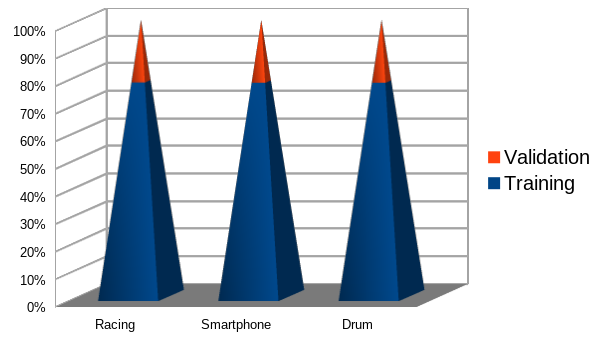
\includegraphics[width=\linewidth]{img/d_s}
     \caption{Relative Train-Validation distribution of each class in our dataset.}\label{Fig:Data1}
   \end{minipage}\hfill
   \begin{minipage}{0.35\textwidth}
     \centering
     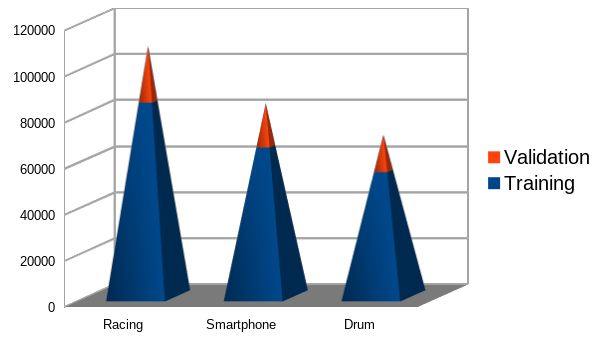
\includegraphics[width=\linewidth]{img/d}
     \caption{Train-Validation distribution of each class by numbersin our dataset.}\label{Fig:Data2}
   \end{minipage}\hfill
   \begin{minipage}{0.29\textwidth}
     \centering
     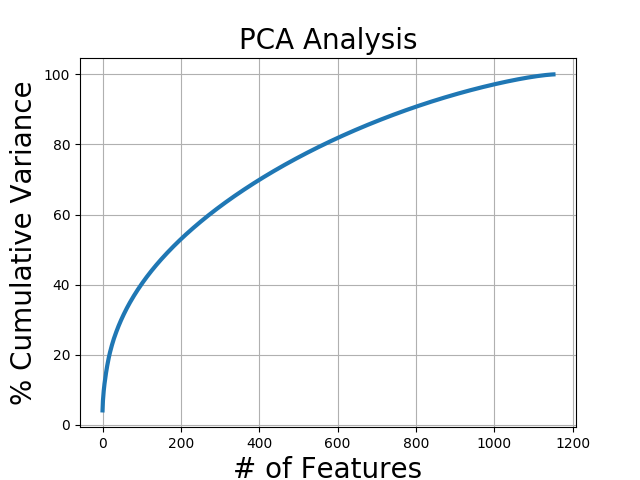
\includegraphics[width=\linewidth]{img/PCA_Analysis}
     \caption{PCA analysis.}\label{fig:pca}
   \end{minipage}
\end{figure}


In order to extract the previous features we parse all tensorflow protocol buffer files (which is a special representation of data in order to store it physically) and for each, we first extract the label and compare it into our provided list of labels. If the former matches our choice, we parse the set of features and append them into an output file on the hard drive otherwise, just skip the record. The final representation of the data is a Comma Separated Values (CSV) containing 1152 features (columns) and a label. Files are eventually available publicly\footnote{\url{https://owncloud.tuwien.ac.at/index.php/s/OB60wk49xzhj398}}.

\begin{figure}[!ht]
\centering
% -------------- SUBFIGURE -1 -------------- %
\begin{subfigure}[Angle 1 of the input space.]{
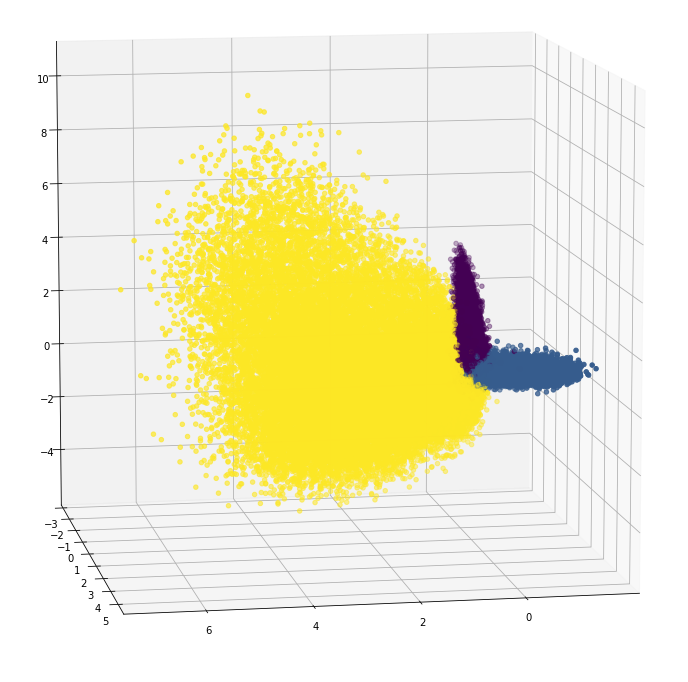
\includegraphics[width=.3\linewidth] {img/movie80}   
\label{fig:pca1} }
\end{subfigure}
\hfill
% -------------- SUBFIGURE -2 -------------- %
\begin{subfigure}[Angle 2 of the input space.]{
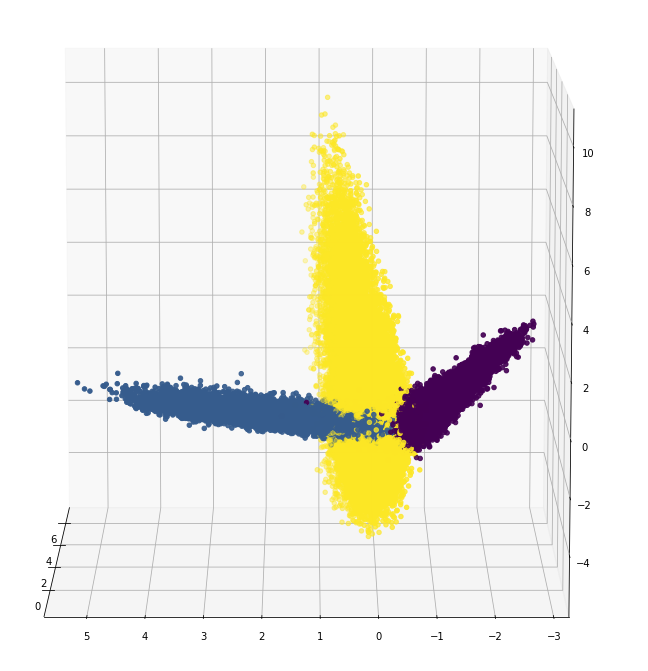
\includegraphics[width=.3\linewidth] {img/movie180}
\label{fig:pca2} }%
\end{subfigure}
\hfill
% -------------- SUBFIGURE -3 -------------- %
\begin{subfigure}[Angle 3 of the input space.]{
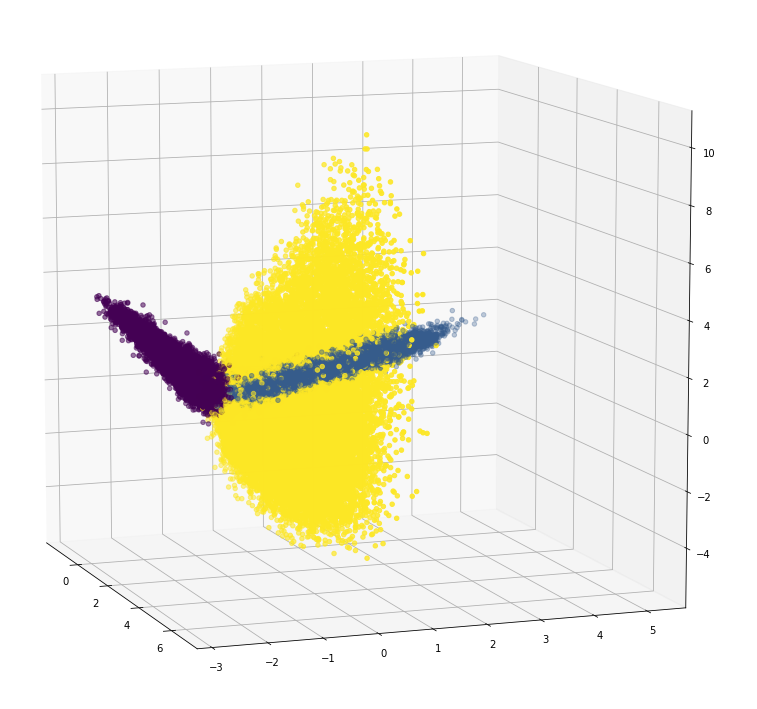
\includegraphics[width=.3\linewidth] {img/movie340}
\label{fig:pca3} }%
\end{subfigure}%

\label{fig:reduction}                            % label to the whole figure
\caption{The new input space after PCA. the three classes are easily separable.}
\end{figure}



We proceed next to the dimentionnality reduction, we chose two basic techniques:
\begin{itemize}
\item First, we convert the original space into a rotated space by maximizing the variance in the first few dimensions, this can be achieved by using Principal Component Analysis (PCA). Figure \ref{fig:pca} show the accumulative variance distribution of all components. After experimenting, we noticed that the first 3 dimensions contains 15\% of the information but represent the data perfectly. Figures \ref{fig:pca1}, \ref{fig:pca2} and \ref{fig:pca3} show the reduced space and the colors represents the three classes. It is worth to mention the the data is scaled before performing PCA.

\item The second option is Random Forests (RF) feature importance metric which is a measure for how pure a feature is (in other words, features with higher split in the tree get higher importance). Applying this technique and removing features with vanishing importance let us reduce the dimension from the raw dataset, however this technique is unexplainable, we tried it at first bu we opted only for PCA at the end.
\end{itemize}

One of the decisions we had to make here is the order of reduction/selection. We applied only PCA since the resulting three dimensions meet our needs and there is no need for further reduction.

Additionally, it is worth to mention that ANNs are able to learn the feature importance without the previous steps however, if we aim for a fair comparison, we feed the same data to all algorithms. Moreover, the higher the dimension is, the more risk we have to over-fit. Actually, in our case we tried with the full dataset at first but it turns out that all our models strongly over-fit hence, we decided to loos information for the sake of reducing over-fitting.

Moreover, the resulting three dimension are not generic meaning that other types/classes of videos might not be well represented in our space but for this task, the later should be sufficient.


\section{Experiments}

The framework used for the classification task is rather simple. Figure \ref{fig:framework} show the different stages used in order to evaluate each classifier. We first start by feeding the scaled training set and training labels into the algorithm under test. A 5-fold cross-validation scheme is applied in order to generalize the performance of each model by monitoring the accuracy of each fold. In addition, a parameter tuning step is optionally added in which the algorithm's parameters are tuned using evolutionary search for better performance (the evolutionary search uses genetic algorithms to get the best performing child). After performing the cross-validation, a fully working model is obtained utilizing the same previous architecture however this time by training it with the whole training data. The former model is then used to predict classes of \textbf{unseen} data sample from the validation set as well as data samples from the training set which results in two sets of predictions. Finally, we compute confusion matrices for both training and validation sets using the ground-truth provided with the validation set. We use three supervised learning metrics for the evaluation: Accuracy, weighted F1-score and weighted Jaccard index.

It is worth to mention that the labels were additionally preprocessed for a few algorithms. For instance, ANNs and multi-class Least Squares need a three dimensional target vector so the raw labels were converted into dummy variables, meaning that a single column of labels is converted into a multi-column binary output.

For reproducibility purposes, all scripts used for preprocessing, training and testing are available in the personal github repository\footnote{\url{https://github.com/fm94/itmlwa}}.

\subsection{parametrisation}
We discuss here briefly the configuration of each algorithm.

\paragraph{Artificial Neural Networks}
The architecture used consist of an input layer with the same dimension as the input data, 9 neuron and 16 neurons hidden layers with \emph{relu} activation functions and batch normalization and finally a three neurons output layer with a sigmoid activation (we used sigmoid here to obtain probabilities since we wanted to investigated the confidence). The choice of the number of layers and number of neurons is arbitrary. Moreover, we use 30\% dropout after the first hidden layer to reduce the dependence of the network on some neurons since we expected a large over-fitting due to the lake of the training data. Moreover, we use 20 training epoch with a batch size of 32 and early stopping if the validation loss does not change by $10^{-6}$ for three epochs. For the back-propagation, we use an adam optimizer with the categorical cross-entropy loss function to train the network and we monitor the accuracy score after each epoch.

\paragraph{Naive Bayes}
For this classifier we use a Gaussian Naive Bayes without any parametrisation and without any prior probabilities. We furthermore, assume that the features are uncorrelated (since they were already extracted from a deep network and PCA were applied afterwards) which is an important assumption for a NB classifier to work.

\paragraph{Random Forests}
We tune two of the RF parameters: maximum depth of the tree and the minimum samples needed to create a leaf, we find respectively 12 and 6 after 6 generation and 300 combinations of a genetic search. Moreover, we use a set of 10 trees in the forest. In order to measure the quality of splits, we use the gini impurity.

\paragraph{Support Vector Machine}
The only parameter that we use in this classifier in the sigmoid kernel under the assumption that a linear kernel cannot separate the space perfectly. The penalty parameter is kept as 1 and we did not tune the parameters since SVM classifiers are known to be computationally heavy.

\paragraph{k-Nearest Neighbor}
We tune the algorithm and found that 10 nearest neighbors is the best parameter for finding the class of a new data point. The distance used is the euclidean distance, this again should be avoided in high dimensional data since the euclidean distance is proved to show unexpected behavior however, since we are dealing with three dimensions, it is fine to use it.

\paragraph{Multi-class Least Squares}
There were no parameters to tune in this case. 
Since the multi-class least squares classification is not implemented in well know libraries, we use a python implementation\footnote{\url{https://github.com/HarryGogonis/Python-Linear-Least-Squares-Classifier}} and improve it. In general, the idea is to find the weights that is in this case not a vector but a matrix that contains three dimensions, one for each class. Later on, the class of a new data sample $\underline{x}$ is estimated by computing $\widehat{\underline{y}} = argmax \widehat{\textbf{W}}^{T}\underline{x}$ and taking the argument of the maximum value.

\begin{figure}
\center
  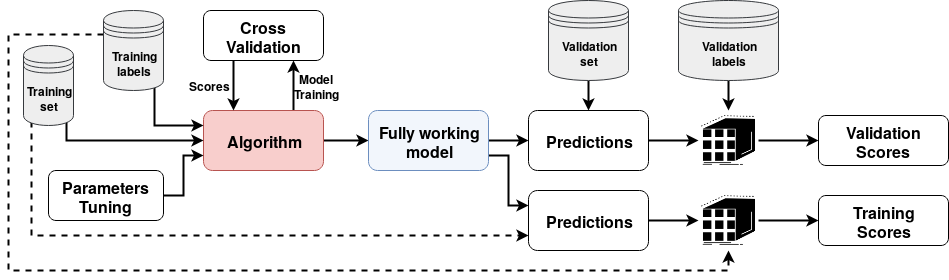
\includegraphics[width=0.9\linewidth]{img/framework}
  \caption{Analysis framework.}
  \label{fig:framework}
\end{figure}


\section{Results and Discussions}
We start by observing the cross-validation scores of the training set. Table \ref{tab:cv} show the average accuracy score with the standard deviation of each algorithm. As a baseline, the majority random guessing accuracy score is ~70\% which is the best score that we can get randomly.

Interestingly, KNN perform the best during the training cross-validation with even a low standard deviation. ANN, RF performed similar and slightly worst than KNN, NB show lower performance followed by SVM and finally LS which was expected since the problem is not totally linearly separable. The NB classifier was expected to perform worst however the fact the PCA was applied before classification, the former reinforced the assumption of independent features which improves the performance of the NB classifier.

\begin{table}
\center

\begin{tabular}{l*{6}{c}r}
Data           & ANN & NB & RF & SVM & kNN & LS \\
\hline
Training Set          & 0.967  & 0.929   & 0.968  & 0.905  & 0.970  & 0.846  \\
& (+/- 0.006) & (+/- 0.001) & (+/- 0.001) & (+/- 0.002) & (+/- 0.001) & (+/- 0.004) \\

\end{tabular}
\caption{Cross-Validation accuracy scores.}
\label{tab:cv}
\end{table}

We move on the the confusion matrices, time time we show a set of twelve confusion matrices representing six algorithms and both training and validation sets in Figure \ref{fig:cms}.

\begin{figure}[!ht]
\centering
% -------------- SUBFIGURE -1 -------------- %
\begin{subfigure}[Training set performance with an Artificial Neural Network model.]{
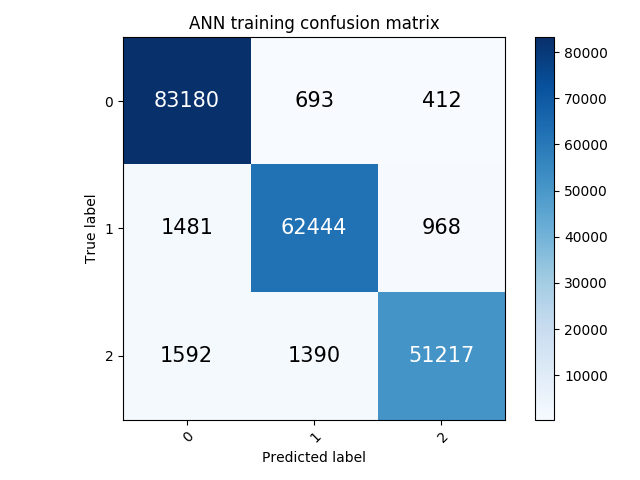
\includegraphics[width=.3\linewidth] {img/ANN_tr_cm}   
\label{fig:subfig1} }
\end{subfigure}
\hfill
% -------------- SUBFIGURE -2 -------------- %
\begin{subfigure}[Training set performance with a Naive Bayes model.]{
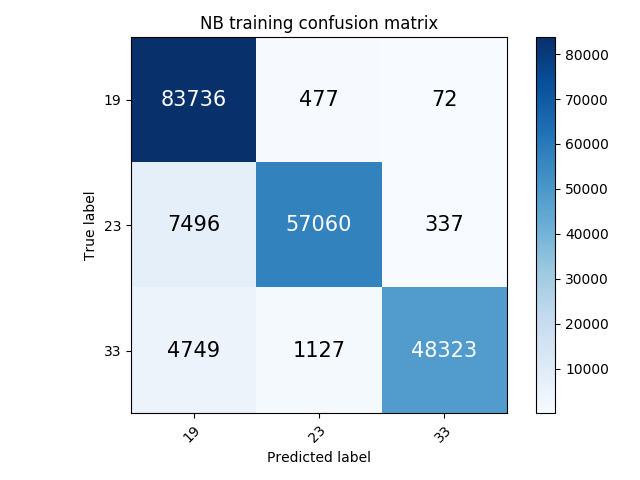
\includegraphics[width=.3\linewidth] {img/NB_tr_cm}
\label{fig:subfig2} }%
\end{subfigure}
\hfill
% -------------- SUBFIGURE -3 -------------- %
\begin{subfigure}[Training set performance with a Random Forests model.]{
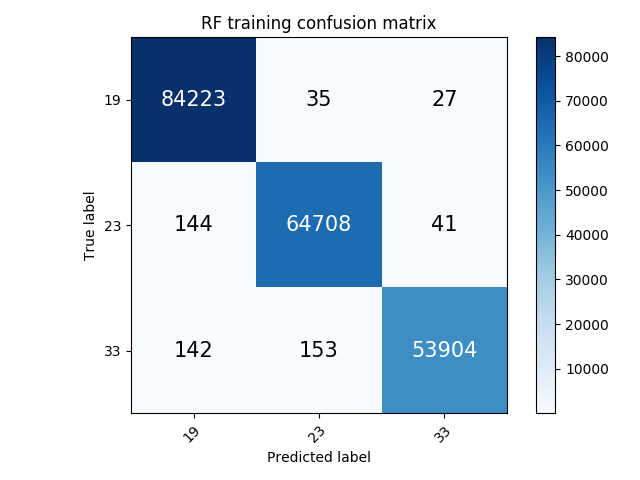
\includegraphics[width=.3\linewidth] {img/RF_tr_cm}
\label{fig:subfig3} }%
\end{subfigure}%
\hfill
% -------------- SUBFIGURE -1 -------------- %
\begin{subfigure}[Validation set performance with an Artificial Neural Network model.]{
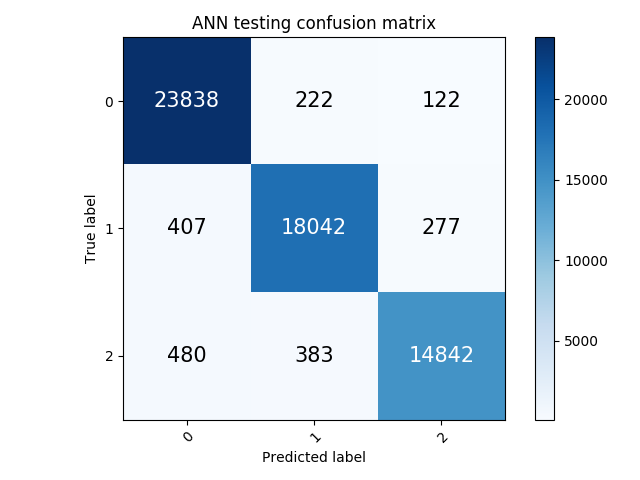
\includegraphics[width=.3\linewidth] {img/ANN_ts_cm}   
\label{fig:subfig1} }
\end{subfigure}
\hfill
% -------------- SUBFIGURE -2 -------------- %
\begin{subfigure}[Validation set performance with a Naive Bayes model.]{
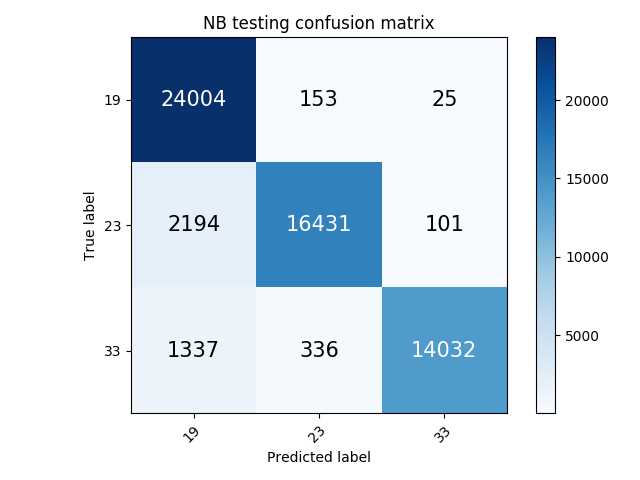
\includegraphics[width=.3\linewidth] {img/NB_ts_cm}
\label{fig:subfig2} }%
\end{subfigure}
\hfill
% -------------- SUBFIGURE -3 -------------- %
\begin{subfigure}[Validation set performance with a Random Forests Network model.]{
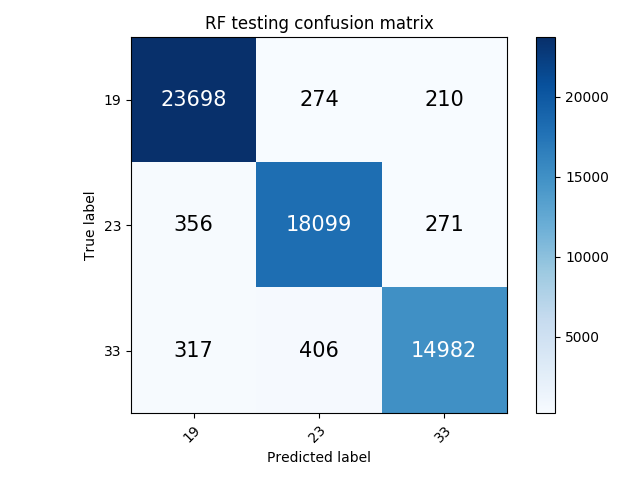
\includegraphics[width=.3\linewidth] {img/RF_ts_cm}
\label{fig:subfig3} }%
\end{subfigure}%
\hfill
% -------------- SUBFIGURE -1 -------------- %
\begin{subfigure}[Training set performance with a Support Vector Machine model.]{
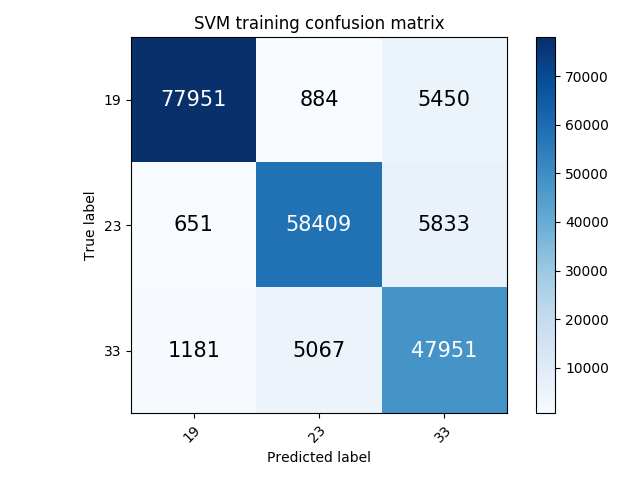
\includegraphics[width=.3\linewidth] {img/SVM_tr_cm}   
\label{fig:subfig1} }
\end{subfigure}
\hfill
% -------------- SUBFIGURE -2 -------------- %
\begin{subfigure}[Training set performance with a K-Nearest Neighbor model.]{
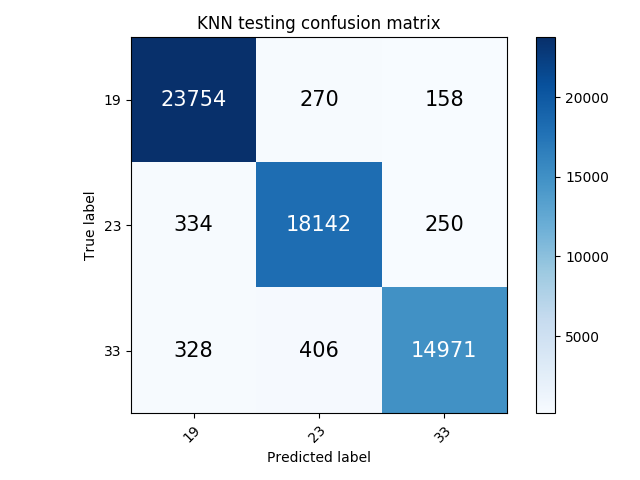
\includegraphics[width=.3\linewidth] {img/KNN_ts_cm}
\label{fig:subfig2} }%
\end{subfigure}
\hfill
% -------------- SUBFIGURE -3 -------------- %
\begin{subfigure}[Training set performance with a Least Squares model.]{
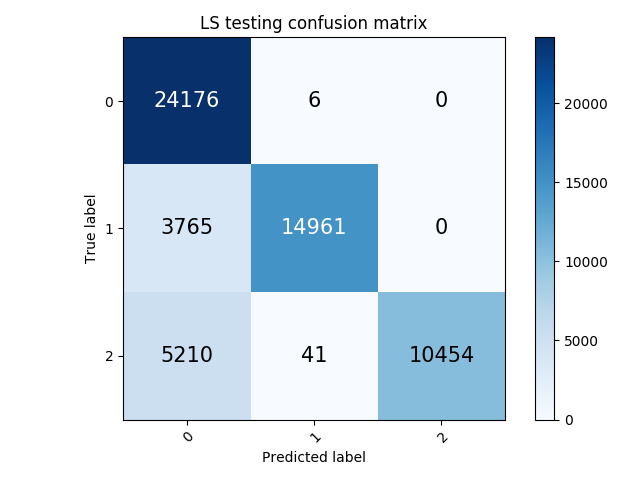
\includegraphics[width=.3\linewidth] {img/LS_ts_cm}
\label{fig:subfig3} }%
\end{subfigure}%
\hfill
% -------------- SUBFIGURE -1 -------------- %
\begin{subfigure}[Validation set performance with a Support Vector Machine model.]{
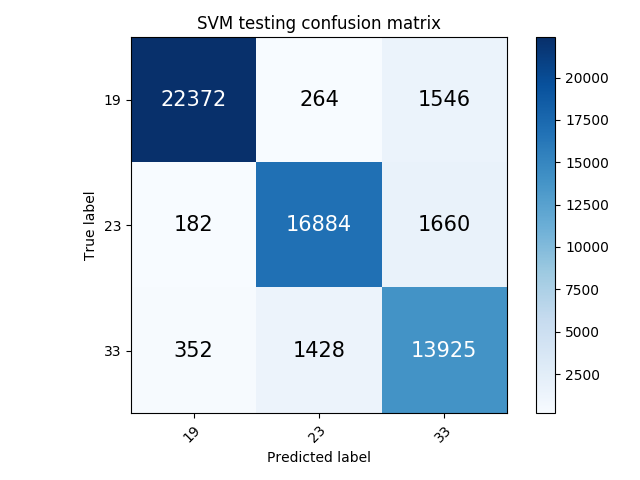
\includegraphics[width=.3\linewidth] {img/SVM_ts_cm}   
\label{fig:subfig1} }
\end{subfigure}
\hfill
% -------------- SUBFIGURE -2 -------------- %
\begin{subfigure}[Validation set performance with a K-Nearest Neighbor model.]{
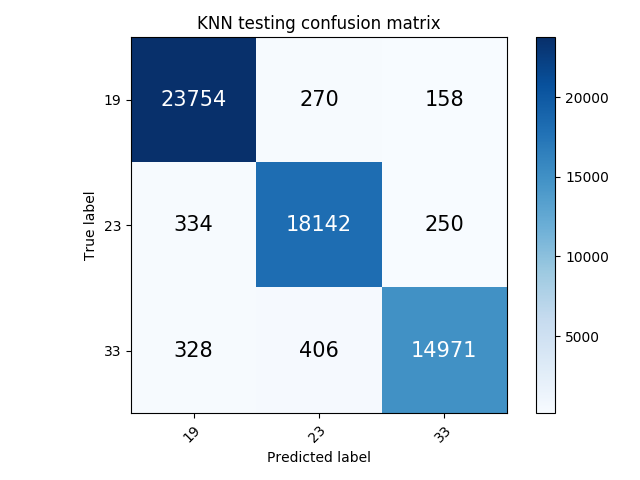
\includegraphics[width=.3\linewidth] {img/KNN_ts_cm}
\label{fig:subfig2} }%
\end{subfigure}
\hfill
% -------------- SUBFIGURE -3 -------------- %
\begin{subfigure}[Validation set performance with a Least Squares model.]{
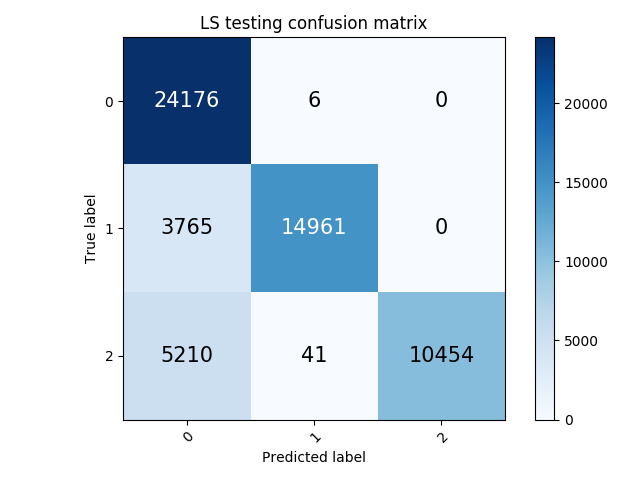
\includegraphics[width=.3\linewidth] {img/LS_ts_cm}
\label{fig:subfig3} }%	
\end{subfigure}%
\hfill
 
\label{fig:cms}                            % label to the whole figure
\caption{Confusion matrices of different models.}
\end{figure}

A few things that we can observer from the confusion matrices are:
\begin{itemize}


\item The first phenomena to notice is the diagonality of the matrices. The former reflect a collection of good classifiers since a diagonal confusion matrix means less False Positives and False Negatives. However, in any case, many samples were miss-classified in the case all algorithms.

\item The second phenomena is that the training set always performs better that the validation set. This is quite intuitive since any algorithm is able to better classifier data samples that it has seen before. Despite the fact that predicting classes of the training data is useless in practice, the former gives us an idea on the generalization of our model.

\item The third phenomena that we notice is that RF performed extremely well on the training set but the poorly for the validation set. This is a well known property of RF since during training the trees tend to over-fit if the the maximum depth is large (12 in our case). As mentioned before, we opt for the cross-validation to reduced the over-fitting.

\item The last phenomena that we notice is triangular confusion matrix in the case of LS classification. The explanation is rather strait forward: the hyper-planes created by the LS estimation moves toward the larger cluster (yellow) in Figure \ref{fig:reduction} thus, all misclassified instances lay only on one half of the confusion matrix. This exactly meets the theory discussed during the course.


\end{itemize}

Finally, we show three metrics extracted from the previous confusion matrices for both the training set and validation set in Figure \ref{fig:comparison1} and Figure \ref{fig:comparison2} respectively. The previous conclusions hold here as well, RF performed extremely well on the training set but poorly on the validation set where KNN won. LS show the worst performance.

If we would make a list of the best classifiers based on the validation set then: \textbf{(1) KNN, (2) RF, (3) ANN, (4) NB, (5) SVM, (6) LS.}
 



\begin{figure}[!htb]
\center
   \begin{minipage}{0.5\textwidth}
     \centering
     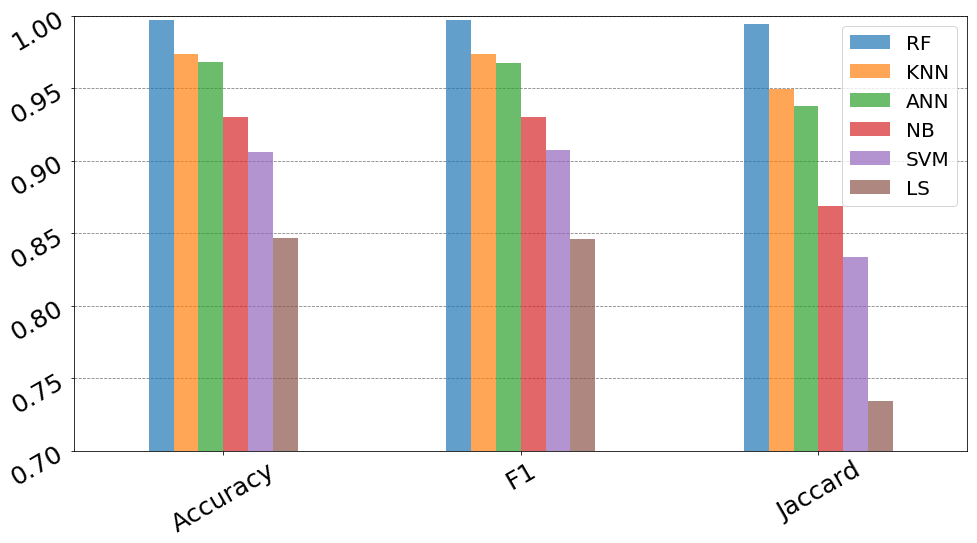
\includegraphics[width=\linewidth]{img/comparison1}
     \caption{Training set scores.}\label{fig:comparison1}
   \end{minipage}%\qquad
   \begin{minipage}{0.5\textwidth}
     \centering
     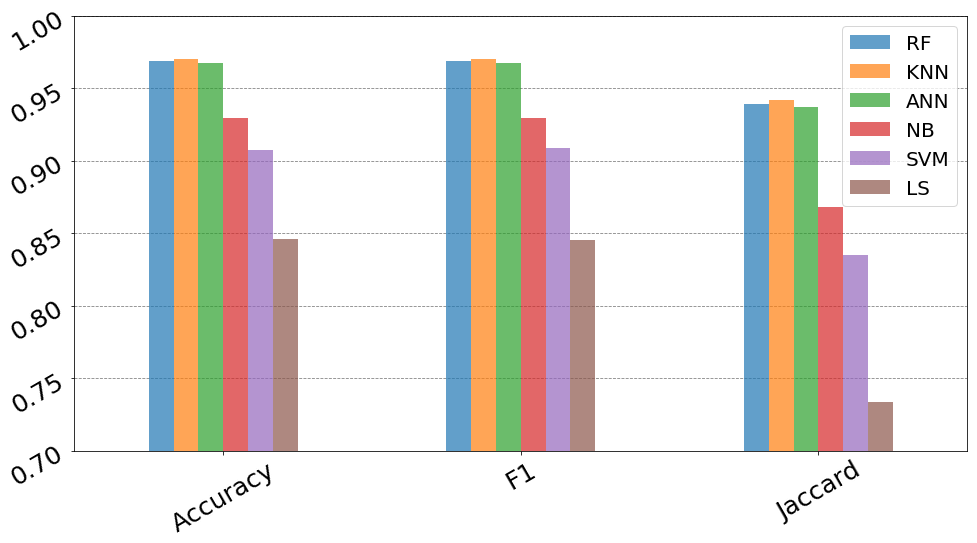
\includegraphics[width=\linewidth]{img/comparison2}
     \caption{Validation set scores.}\label{fig:comparison2}
   \end{minipage}
\end{figure}



\section{Conclusion}
In this work, we created a benchmark to compare the performance of six classification algorithms for predicting videos labels in a supervised manner. We filtered out three classes from the well known Youtube-8M dataset. Moreover, in order to reduce the dimensionality, we opt for PCA feature reduction technique and reduced the dimension to only \textbf{three} dimensions. In order to evaluate our algorithms, a cross-validation in addition to a comparative study is carried out. Three metrics (Accuracy, F1 score and Jaccard score) were extracted from the confusion matrices and compared.

Results suggest that most models performed extremely good except the Naive Bayesian approach. However, we believe that the classes that were chosen (Racing, Smartphones and Drum) are easily separable and far from each other in the input space, this is one of the reasons that allows us to reduce the dimension of the input space and later on led us into high prediction scores. In fact, we tried many classes combinations before with which the performance were worst than a random guessing classification.

The fact that features were extracted from well known powerful architectures let us assume that the data is already well represented and for sure, dealing with raw videos would be way much harder.

We note that in earlier experiments with much more dimensions, all classifiers over-fitted. This is obvious since the larger the dimension is, the more training data we need so we tried to make the problem harder by removing considerable amount of information by applying PCA.

Finally, we prove that no matter which approach one takes to solve such real problems, with the same complexity the results should almost always be similar and no magic is included in the formula.
 
 
%----------------------------------------------------------------------------------------
%	BIBLIOGRAPHY
%----------------------------------------------------------------------------------------

\bibliographystyle{apalike}

\bibliography{sample}

%----------------------------------------------------------------------------------------


\end{document}